\documentclass[11pt, oneside]{article} 
\usepackage{geometry}
\geometry{letterpaper} 
\usepackage{graphicx}
	
\usepackage{amssymb}
\usepackage{amsmath}
\usepackage{parskip}
\usepackage{color}
\usepackage{hyperref}

\graphicspath{{/Users/telliott_admin/Dropbox/Tex/png/}}
% \begin{center} 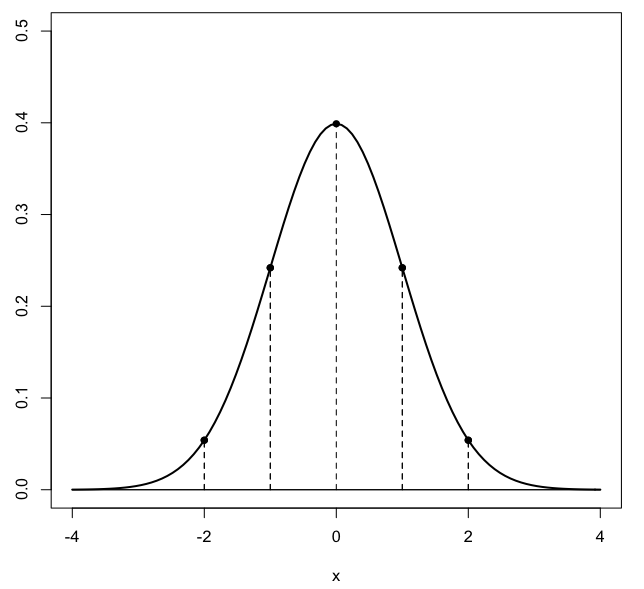
\includegraphics [scale=0.4] {gauss3.png} \end{center}

\title{Brilliant wiki}
\date{}

\begin{document}
\maketitle
\Large
I found another derivation here:

\url{https://brilliant.org/wiki/deriving-keplers-laws/}

We start with Newton's second law:
\[ \mathbf{F} = m\mathbf{a} \] 
where $\mathbf{a}$ describes the acceleration, which in radial coordinates is $\ddot{\mathbf{r}}$.
By hypothesis, the force is
\[ \mathbf{F} = - \frac{GmM}{r^2} \ \hat{\mathbf{r}} \]
To solve this, convert to Cartesian $xy$-coordinates, breaking the acceleration into two components
\[ m \ddot{\mathbf{x}} = - \frac{GmM}{r^2} \cos \theta \]
\[ m \ddot{\mathbf{y}} = - \frac{GmM}{r^2} \sin \theta \]

We will use a trick to solve the system.  Getting ahead of ourselves a little bit, cancel the $m$, and multiply the first equation by $\cos \theta$ and the second by $\sin \theta$:
\[ \ddot{\mathbf{x}} \cos \theta = - \frac{GM}{r^2} \cos^2 \theta \]
\[ \ddot{\mathbf{y}} \sin \theta = - \frac{GM}{r^2} \sin^2 \theta \]
then add
\[ \ddot{\mathbf{x}} \ \cos \theta + \ddot{\mathbf{y}} \ \sin \theta = - \frac{GM}{r^2} \]
We will provide another equality involving the left-hand side.

\subsection*{derivatives}
According to the source:  "we need to find the second derivative of the $x$ and $y$ coordinates in terms of the polar coordinates."  Repeat what we've done elsewhere:
\[ x = r \cos \theta \]
\[ \dot{x} = \dot{r} \cos \theta - r \dot{\theta} \sin \theta \]
By the chain rule.  Notice there are three components in the second term.
\[ \ddot{x} = \ddot{r} \cos \theta - \dot{r}  \dot{\theta} \sin \theta - \ [ \ \dot{r} \dot{\theta} \sin \theta + r \ddot{\theta} \sin \theta +   r \dot{\theta}^2 \cos \theta \ ] \]
\[ = \ddot{r} \cos \theta - 2 \dot{r}  \dot{\theta} \sin \theta - r \ddot{\theta} \sin \theta - r \dot{\theta}^2 \cos \theta \]
It looks like a mess, but it will all work out.  Next:
\[ y = r \sin \theta \]
\[ \dot{y} = \dot{r} \sin \theta + r \dot{\theta} \cos \theta \]
\[ \ddot{y} = \ddot{r} \sin \theta + \dot{r} \dot{\theta} \cos \theta + \ [ \ \dot{r} \dot{\theta} \cos \theta + r \ddot{\theta} \cos \theta - r \dot{\theta}^2 \sin \theta  \ ]  \]
\[ = \ddot{r} \sin \theta + 2 \dot{r} \dot{\theta} \cos \theta + r \ddot{\theta} \cos \theta - r \dot{\theta}^2 \sin \theta  \]
Now, when we multiply the equation for $\ddot{x}$ by $\cos \theta$, there are two terms with $\sin \theta \cos \theta$:
\[ \dots - 2 \dot{r}  \dot{\theta} \sin \theta \cos \theta - r \ddot{\theta} \sin \theta \cos \theta \dots \]

which exactly cancel the second and third terms from the expression for $\ddot{y}$, multiplied by $\sin \theta$, when the two parts are added together.  

We obtain:
\[ \ddot{\mathbf{x}} \ \cos \theta + \ddot{\mathbf{y}} \ \sin \theta = \]
\[ = \ddot{r} \cos^2 \theta - r \dot{\theta}^2 \cos^2 \theta +  \ddot{r} \sin^2 \theta - r \dot{\theta}^2 \sin^2 \theta  \]
\[ = \ddot{r}  - r \dot{\theta}^2 \]
which you must admit is an impressive simplification.  

Combining with the previous result we have:
\[  \ddot{r}  - r \dot{\theta}^2 = - \frac{GM}{r^2} \]
Suppose $r$ is constant, then  $\ddot{r} = 0$ and
\[ r \dot{\theta}^2 = \frac{GM}{r^2} \]
We found previously that for a circular orbit
\[ v = \sqrt{\frac{GM}{R}} \]
\[ \frac{v^2}{R} = \frac{GM}{R^2} \]
But $v = R\omega = R \dot{\theta}$.  This is the same equation.

\subsection*{Kepler 2}
Rather than multiply as we did, switch and multiply $\ddot{x}$ by $\sin \theta$ and $\ddot{y}$ by $\cos \theta$:
\[ \ddot{x} \sin \theta = \ddot{r} \sin \theta \cos \theta - 2 \dot{r}  \dot{\theta} \sin^2 \theta - r \ddot{\theta} \sin^2 \theta - r \dot{\theta}^2 \sin \theta \cos \theta \]
\[ \ddot{y} \cos \theta = \ddot{r} \sin \theta \cos \theta + 2 \dot{r} \dot{\theta} \cos^2 \theta + r \ddot{\theta} \cos^2 \theta - r \dot{\theta}^2 \sin \theta \cos \theta  \]
And subtract:
\[ \ddot{x} \sin \theta - \ddot{y} \cos \theta = - 2 \dot{r}  \dot{\theta} - r \ddot{\theta} \]
But the left-hand side is zero (go back to the original equation)
\[ 0 = - 2 \dot{r}  \dot{\theta} - r \ddot{\theta} \]
\[ 2 \dot{r}  \dot{\theta} + r \ddot{\theta} = 0 \]
Multiply by $r$ and recognize
\[ 2 r \dot{r}  \dot{\theta} + r^2 \ddot{\theta} = 0 = \frac{d}{dt} \ r^2 \dot{\theta} \]

$m$ times this quantity whose derivative is zero is the angular momentum.  Hence the angular momentum is conserved.  Multiply by $m$ and integrate with respect to time:
\[ L = mr^2 \dot{\theta} \]
Integrate again with respect to time:
\[ \frac{L}{m} t = \int r^2 \theta \]
The quantity on the right-hand side is twice the area swept out from $\theta_1$ to $\theta_2$, which is now seen to be independent of $r$ (since it is equal to a constant times the time).

\subsection*{Kepler 1}
In the first section, we had
\[  \ddot{r}  - r \dot{\theta}^2 = - \frac{GM}{r^2} \]
We must now solve this equation.  Substitute $u = 1/r$.
\[ \dot{r} = \frac{dr}{dt} = -\frac{1}{u^2} \ \frac{du}{dt} = -\frac{1}{u^2} \ \frac{du}{d \theta} \ \dot{\theta}  \]
And recalling the previous result:
\[ \frac{L}{mr^2} = \dot{\theta} = \frac{L}{m}u^2 \]

So substitute for $\dot{\theta}$ in the equation with $u$:
\[ = -\frac{1}{u^2} \ \frac{du}{d \theta} \ \frac{L}{m} u^2 \]
\[= -\frac{L}{m} \ \frac{du}{d \theta}  \]
Differentiating again:
\[ \ddot{r} = -\frac{L}{m} \ \frac{d}{dt} \ ( \frac{du}{d \theta} ) \]
\[ \ddot{r} = -\frac{L}{m} \ \frac{d \theta}{dt} \ \frac{d}{d \theta} \ ( \frac{du}{d \theta} ) \]
(By the chain rule).

Substituting again for $\dot{\theta}$
\[ \ddot{r} = - (\frac{L}{m})^2 \ u^2 \ \frac{d^2u}{d \theta^2} \]

Go back to 
\[  \ddot{r}  - r \dot{\theta}^2 = - \frac{GM}{r^2} \]
and substitute:
\[ - (\frac{L}{m})^2 \ u^2 \ \frac{d^2u}{d \theta^2} - \frac{1}{u} \ [ (\frac{L}{m})u^2]^2  = - GMu^2\]
\[ - (\frac{L}{m})^2 \ \frac{d^2u}{d \theta^2} - (\frac{L}{m})^2u  = - GM\]
\[ - \frac{d^2u}{d \theta^2} + GM (\frac{m}{L})^2   = u \]

$u$ is just a periodic function of $\theta$.
\[ u = A \cos ( \theta + \delta) + C \]
where $C = GMm^2/L^2$. 
We can always define coordinates such that $\delta = 0$ so
\[ u = A \cos \theta + C \]
\[ r = \frac{1}{A \cos \theta + C} \]
\[ = \frac{1}{C (A/C \cos \theta + 1)} \]
With an appropriate definition ($e = A/C$) we can write
\[ r = \frac{e/A}{ e \cos \theta + 1} \]

This is the equation of an ellipse in radial coordinates.  The closest and furthest approaches occur when $\theta = 0, \pi$ and then 

\[ r = \frac{e/A}{ 1 \pm e} \]
The semi-major axis is 
\[ a = \frac{1}{2}(r_{min} + r_{max}) \]
\[ = \frac{e/a}{1 - e^2} \]

\end{document}  